\documentclass{beamer}

\usepackage[english]{babel}
\usepackage{graphicx,hyperref,ru}

% A few hacks to get references via bibtex (easy reuse for paper)
\usepackage{bibentry}
\nobibliography*
\let\newblock\relax
\setbeamertemplate{bibliography item}{}

\title{Privacy in Cloud Computing}

\author{Aram Verstegen \and Erik Boss}

\institute{Radboud University Nijmegen}

\date{\today}

\begin{document}

\begin{frame}
  \titlepage
\end{frame}

\begin{frame}
  \frametitle{Outline}
  \tableofcontents
\end{frame}

% These frametitles are kinda tongue-in-cheek, not sure if I want to keep them -- Erik

\section{Introduction}
% I estimate this section at about 20 minutes (depending on amount questions)

\begin{frame}
  \frametitle{Outline}
  \tableofcontents[currentsection,currentsubsection]
\end{frame}

\begin{frame}
    \frametitle{What are we dealing with?}
    %/* General definitions, explanations on cloud computing: SaaS/PaaS/IaaS
    %(with a picture?), public/private/community/hybrid clouds  */
    \begin{itemize}
        \item Software as a Service (SaaS) \\
            Webmail, online storage, social media
        \item Platform as a Service (PaaS) \\
            Virtual application platforms
        \item Infrastructure as a Service (IaaS) \\
            Scalable computing and storage services
        \item Test: \bibentry{takabi2010security} % remove after real references added in
    \end{itemize}
\end{frame}

\begin{frame}
    \frametitle{A picture is worth\dots}
    \begin{figure}
        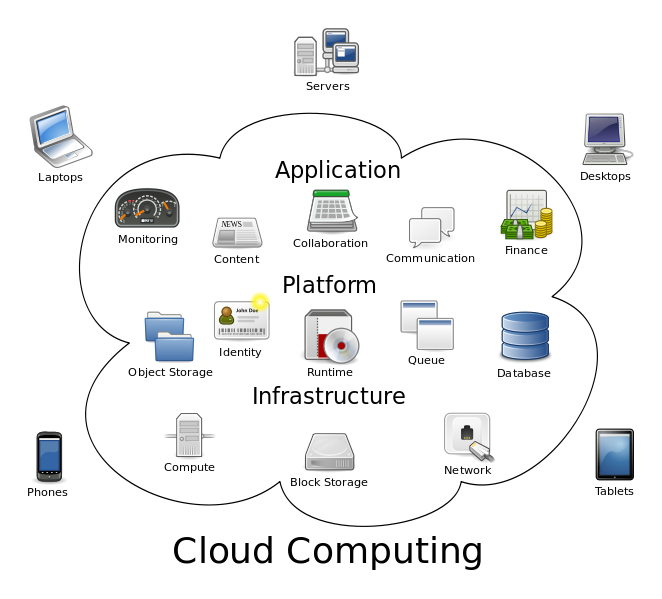
\includegraphics[height=\textheight]{../img/cloudoverview.png}
        \label{fig:cloudoverview}
    \end{figure}
\end{frame}

\begin{frame}
    \frametitle{Whom are we dealing with?}
    \only<1>{
    Roles:
    \begin{itemize} % We might put this in a pyramid diagram
        \item Cloud service providers that offer XaaS
        \item Cloud service users that build services on said service
        \item Customers of these services
    \end{itemize}
    }

    \only<2>{
    Cloud Service providers:
    \begin{itemize}
    \item SaaS \\
        (Google, Apple, Microsoft)
    \item PaaS \\
        (Google AppEngine, Amazon AWS, Microsoft Azure (SQL), EngineYard,
        Heroku)
    \item IaaS \\
        (Amazon EC2 / S3, Google Compute Engine / BigQuery, Linode)
    \end{itemize}
    }
    % Cloud service users: some sites you use, customers: you
\end{frame}

\begin{frame}
    \frametitle{Why does the industry like it?}
    %/* Why use cloud computing at all; virtualization, scaling, fast
    %deployment, pay-for-use, etc  */
    \begin{itemize}
        \item Cost
        \item Fast wide scalability
        \item Pay as you go
        \item Outsource responsibility
        \item Has better security than most providers
        \item Buzz
    \end{itemize}
\end{frame}

\begin{frame}
    \frametitle{Why should we be skeptical?}
    %/* What are the problems; general overview of the security requirements and
    %problems (depending on type of cloud); picture(s) about cloud security for
    %fun and profit */
    \begin{itemize}
        \item Centralized assets
        \item Less diversity
        \item Resource sharing (logical segregation)
        \item Usually has better security
        \item But: major impact when breaches do occur
        \item Typical centralized versus decentralized discussion
        \item Faith in the cloud provider?
    \end{itemize}
\end{frame}

\begin{frame}
    \frametitle{Personal data}
    \begin{itemize}
      \item E-mail address
      \item IP address
      \item Username
      \item Password
      \item Banking details
      \item Medical records
    \end{itemize}
\end{frame}

\begin{frame}
    \frametitle{Might your data be in peril?}
    %/* Global overview on specific privacy concerns w.r.t. clouds; example(s)
    %of how things can go badly; primarily: why does it matter! */
    \begin{itemize}
        \item ``Real name policy''
        \item Data ownership
        \item Continuity
        \item Local legislation % For example: age of consent in various countries - flickr picture legal one place, illegal in another
            %\item Piracy claims vs Fair use % (YouTube knows about that song you ripped off and is obliged to tell the authorities)
        \item The declining cost of storing \textbf{everything}
        \item Thus making breaches evermore dangerous, however they occur
        \item Given the ability to analyse large amounts of personal data
        \item SLA/EULA
    \end{itemize}
\end{frame}

\begin{frame}
    \frametitle{Provider viewpoints}
    \begin{itemize}
        \item \textbf{Google}: ``Onze menukaart is beperkt, maar je kunt toch weg? Dan moet
        je verder niet zeiken'' (``Google weigert data in Europa te houden'' -
        Webwereld, 2011)
    \item \textbf{Microsoft}: ``Microsoft cannot provide those guarantees. Neither can
        any other company'' (``Microsoft admits Patriot Act can access EU-based
        cloud data'' - ZDnet, 2011)
    \item \textbf{Amazon}: ``Customers can choose to store all data in the EU by using
        the EU (Ireland) Amazon S3 Region.'' (Amazon S3 FAQ)
    \end{itemize}
\end{frame}

\begin{frame}
    \frametitle{Dude, where's my data}
    Where is our data?
    \begin{itemize}
        \item In general: we do not know
        \item And it is hard to find out
        \item But sometimes we do\dots (OV chipkaart: Talys, France)
    \end{itemize}

    \begin{block}{Essential idea}<2>
    The \emph{cloud} is an abstraction.
    \end{block}
\end{frame}

\section{Legal aspects}
% Another 20 minutes should be doable

\begin{frame}
  \frametitle{Outline}
  \tableofcontents[currentsection,currentsubsection]
\end{frame}

\begin{frame}
    \frametitle{Because a little reminder is always nice}
    %/* Quick recap of the most important and relevant legislation, i.e., data
    %protection and privacy directives. */
    \begin{itemize}
        \item EU Data protection directive 95/46/EC
        \item e-Privacy Directive 2002/58/EC
        \item PATRIOT act
        \item Safe Harbor principle (as per 95/46/EC)
    \end{itemize}

    \begin{itemize}
        \item Data subject
        \item Data controller \checkmark
        \item Data processor \checkmark
    \end{itemize}
    % Data processors have it easier WRT legal requirements
\end{frame}

\begin{frame}
    \frametitle{Ship ahoy!}
    \begin{columns}[t]
        \column{0.5\textwidth}
        US:
        \begin{itemize}
            \item Notice
            \item Choice
            \item Onward Transfer
            \item Security
            \item Data Integrity
            \item Access
            \item Enforcement
        \end{itemize}
        \column{0.5\textwidth}
        EU:
        \begin{itemize}
            \item Fairly and lawfully
            \item Purposeful
            \item Proportional
            \item Data Integrity (accuracy)
            \item Consent
            \item Notice
            \item Access
            \item Choice
            \item Safeguards, safeguards everywhere
        \end{itemize}
    \end{columns}
    % Alleen van toepassing voor overdracht van privedata
    %\begin{scriptsize}

    %\begin{itemize}
        %\item \textbf{Notice} - Individuals must be informed that their data is being collected and about how it will be used.
        %\item \textbf{Choice} - Individuals must have the ability to opt out of the collection and forward transfer of the data to third parties.
        %\item \textbf{Onward Transfer} - Transfers of data to third parties may only occur to other organizations that follow adequate data protection principles.
        %\item \textbf{Security} - Reasonable efforts must be made to prevent loss of collected information.
        %\item \textbf{Data Integrity} - Data must be relevant and reliable for the purpose it was collected for.
        %\item \textbf{Access} - Individuals must be able to access information held about them, and correct or delete it if it is inaccurate.
        %\item \textbf{Enforcement} - There must be effective means of enforcing these rules.
    %\end{itemize}
    %\end{scriptsize}
    %\footnotesize{Source: \url{{http://en.wikipedia.org/wiki/International_Safe_Harbor_Privacy_Principles}}}
\end{frame}

\begin{frame}
    \frametitle{Service Level Agreements (SLAs)}
    \begin{itemize}
    \item Contract law
    \item May require you to:
      \begin{itemize} % http://www.networkworld.com/news/2012/120612-hp-amazon-cloud-264847.html?page=2
        \item occupy two mirrored instances at different datacenters
        \item may allow one of these to go down at points
        \item may give different guarantees for different aspects
      \end{itemize}
    \item Are often unnecessarily vague
    \end{itemize}
    \footnotesize{``Gartner: Amazon, HP cloud SLAs are `practically useless''', NetworkWorld, 2012}
\end{frame}

\begin{frame}
    \frametitle{Accountability beyond data transfer}
    \begin{itemize}
    \item ISO27001
    \item SAS70 % Statement on Auditing Standards
    \item SSAE16 % Statement on Standards for Attestation Engagements
    \item ISAE 3402 % International Standards for Security Engagements
    \item Third party memorandum
    \end{itemize}
\end{frame}

\begin{frame}
    \frametitle{There is more to law than code}
    %/* If we do manage to find relevant case law, put it here */
    Article 29 Working Party - (draft) Opinion on cloud computing
    \begin{itemize}
    \item Legal code for data protection reaffirmed
    \item Concerned about confidentiality integrity, availability, isolation, transparency, 
    \item Advises comprehensive risk analysis before moving to cloud
    \item Consider risks, legal requirements, sensitive data
    \item Actually provides a checklist
    \end{itemize}
\end{frame}

\begin{frame}
    \frametitle{As always: ``it depends''}
    /* Legal analysis differs given the type of cloud computing (so break it
    down), it matters whether we have public or private clouds, IaaS or SaaS,
    etc. */
    % Erik, ik weet niet welke kant je hiermee op wilt - laat ik aan jou over
\end{frame}

\begin{frame}
    \frametitle{National Security Letters}
    \begin{itemize}
    \item Subpoena transactional data
    \item No legal recourse
    \item Come with lifelong gag order
    \item PATRIOT act enabled DHS to send NSLs
    \item 192,499 were filed between 2003 and 2006 \footnote{``A Review of the FBI's Use of National Security Letters'' - US DoJ Inspector General, 2008}
    \item Deemed unconstitutional by SF District Court
    \item Senate bill required for more accountability
    \end{itemize}
\end{frame}

\begin{frame}
    \frametitle{NSL case law: John Doe vs Ashcroft}
    \begin{itemize}
    \item Anonymous ISP (Calyx) gets NSLs summoning all kinds of data
    \item ACLU files first amendment claim against attorney general John Ashcroft
    \item NY District Court deems NSL provisions unconstitutional
    \item Congress allows limited review through the law
    \item Government appeals and gets the case dismissed
    \item Same NY judge considers revised provisions and strikes them down again
    \item Government might still appeal
    \end{itemize}
\end{frame}

% Perhaps this is a good one to encite a discussion
% Sure, so I've moved the discussion slide after this one
\begin{frame}
    \frametitle{Strategic defense consideration}
    \begin{itemize}
      \item Large concentrations of valuable data
      \item hosted on shared infrastructure
      \item (with a broad and deep attack surface)
      \item on a platform that offers tremendous computing capacity
      \item to anybody with a credit card
    \end{itemize}
\end{frame}

\section{Technical aspects}

\begin{frame}
  \frametitle{Outline}
  \tableofcontents[currentsection,currentsubsection]
\end{frame}

\begin{frame}
    \frametitle{Reinventing the wheel}
    %/* Some room for discussion: how does our audience feel about the legal
    %bits and pieces? */
    Just like mainframes?
    \begin{itemize}
    \item Scale
    \item Networked environment
    \item No absolute control
    \item Automatic provisioning
    \item Low barrier to entry
    \end{itemize}
\end{frame}

\begin{frame}
    \frametitle{To trust or not to trust}
    %/* In-depth technical privacy in cloud setting; What does privacy mean in
    %this context, how can it be achieved (in general): all sorts of things are involved
    %(network security, web security, encryption, computing under encryption,
    %etc) */

    Availability: \checkmark \\
    Focus on:
    \begin{itemize}
      \item Confidentiality
      \item Integrity
    \end{itemize}
    We apply:
    \begin{itemize} % Note these are ordered from the most ephemeral to the most real
      \item Identity management
      \item Application security
      \item System \& Network security
      \item Physical security
      \item Hypervisor security % Isn't physical security arguably more 'real' than hypervisor security?
    \end{itemize}
\end{frame}

\begin{frame}
    \frametitle{Identity management}
    Prevent identity fraud:
    \begin{itemize}
      \item Single Sign-On (SSO) outside corporate environments % Maybe not this... but it's related
      \item Multi-factor authentication
      \item Password policies, security questions
      \item VPN connections
      \item SSL validity
      \item Still rests on PKI
    \end{itemize}
\end{frame}

\begin{frame}
    \frametitle{Application security}
    Prevent software abuse:
    \begin{itemize}
      \item Input validation
      \item Secure storage
      \item Avoid logical bugs
      \item Audit logging
      \item Application software patches
    \end{itemize}
\end{frame}

\begin{frame}
    \frametitle{System \& Network Security}
    Prevent network abuse:
    \begin{itemize}
      \item Firewalling
      \item Secure tunnels % Maybe skip this
      \item Airgapped management network
      \item Central audit logging
      \item Intrusion detection services (IDS)
      \item System software patches (fabric management)
    \end{itemize}
\end{frame}

\begin{frame}
    \frametitle{Physical Security}
    Prevent physical entry:
    \begin{itemize}
      \item Fences
      \item Locks
      \item Guards
      \item Cameras
      \item Badges \& Secure doors
      \item Electrically safe fire extinguishers (inert gas)
      \item Redundant power, backup power
      \item Redundant cooling water
    \end{itemize}
\end{frame}

\begin{frame}
    \frametitle{Hypervisor security}
    % This is an awesome paper about backdoored C compilers
    ``Reflections on Trusting Trust'' (Kevin Thompson, 1991) \\
    Modern equivalent: cloudburst exploit \\
    Prevent breaking out of virtual machines:
    \begin{itemize}
      \item Software management
      \item Host-based intrusion detection
      \item Hope for the best
    \end{itemize}
\end{frame}

\begin{frame}
    \frametitle{Cloud attacks}
    %/* Attacks, attacks and more attacks; If possible, frighten the audience!
    %Malicious images, simple(r) web application vulnerabilities, etc */
    \begin{itemize}
      \item Simple bruteforcing cloud apps
      \item Cracking in the cloud (Various) % TODO cite
      \item Gigabit DDoS as a service % 250Mbit/s per node!
      \item Poisoning the well (Harron Meer, 2009)
      \item Stealing licence keys (Harron Meer, 2009)
    \end{itemize}
\end{frame}

\begin{frame}
    \frametitle{Privacy Enhancing Technologies}
    %/* Countermeasures; PETs; best practices; more detailed explanations of
    %systems that give privacy guarantees */
    \begin{itemize}
      \item Only store/transfer encrypted data and let the client encrypt it on their machine
      \item Don't store encryption keys in the cloud
      \item Make use of homomorphic encryption to be able to work with encrypted data
      \item Don't log sensitive data
    \end{itemize}
\end{frame}

\begin{frame}
    \frametitle{Case study: private cyberlocker}
    \begin{itemize}
    \item Secure encrypted data
    \item Deduplication
    \item Key management
    \end{itemize}
\end{frame}

\begin{frame}
    \frametitle{Secure encrypted data}
    \begin{itemize}
    \item Open source design
    \item No use of driver blobs, browser plugins or server-side code
    \item Encryption/decryption only happens in the client
    \item Keys only available on client(s)
    \end{itemize}
\end{frame}

%\begin{frame}
    %\frametitle{Deduplication of encrypted data}
    %Use a checksum of the plaintext leaks information about what is stored.
%\end{frame}

\begin{frame}
    \frametitle{Key management}
    Make backup keys

    Private:
    $k_A = genKey()$
    $k_B = genKey()$
    \dots

    $o = hash(p)$

    Public:
    $o_A = E(o, k_A)$
    $o_B = E(o, k_B)$
    \dots

    $c = E(p,o)$
    % Each file has a different key
    % Low overhead
    % Flexible to add new keys/owners
\end{frame}

\begin{frame}
    \frametitle{What is stored}
    \begin{itemize}
    \item Encrypted blob with metadata, checksum
    \item Plaintext's checksum encrypted with user keys
    \end{itemize}
\end{frame}

\begin{frame}
    \frametitle{Results}
    \begin{itemize}
    \item Usable in public and private cloud
    \item Easy deduplication
    \item Add a new (device key) with your old key
    \item Poor backward security
    \end{itemize}
\end{frame}

\begin{frame}
    \frametitle{I can already see the ending}
    /* Obligatory 'Questions?' slide, possibly with a funny picture. */
\end{frame}

\begin{frame}
    \frametitle{References}
    \bibliography{../references/references}
    \bibliographystyle{plain}
\end{frame}

\end{document}
